\documentclass[varwidth, border=8pt]{standalone}
\usepackage{tikz}
\usepackage{xcolor}
\usepackage{caption}
\captionsetup{justification=raggedright,singlelinecheck=false}
\usetikzlibrary{positioning,arrows,arrows.meta}
\begin{document}

\begin{minipage}{\linewidth}
\begin{center}

    
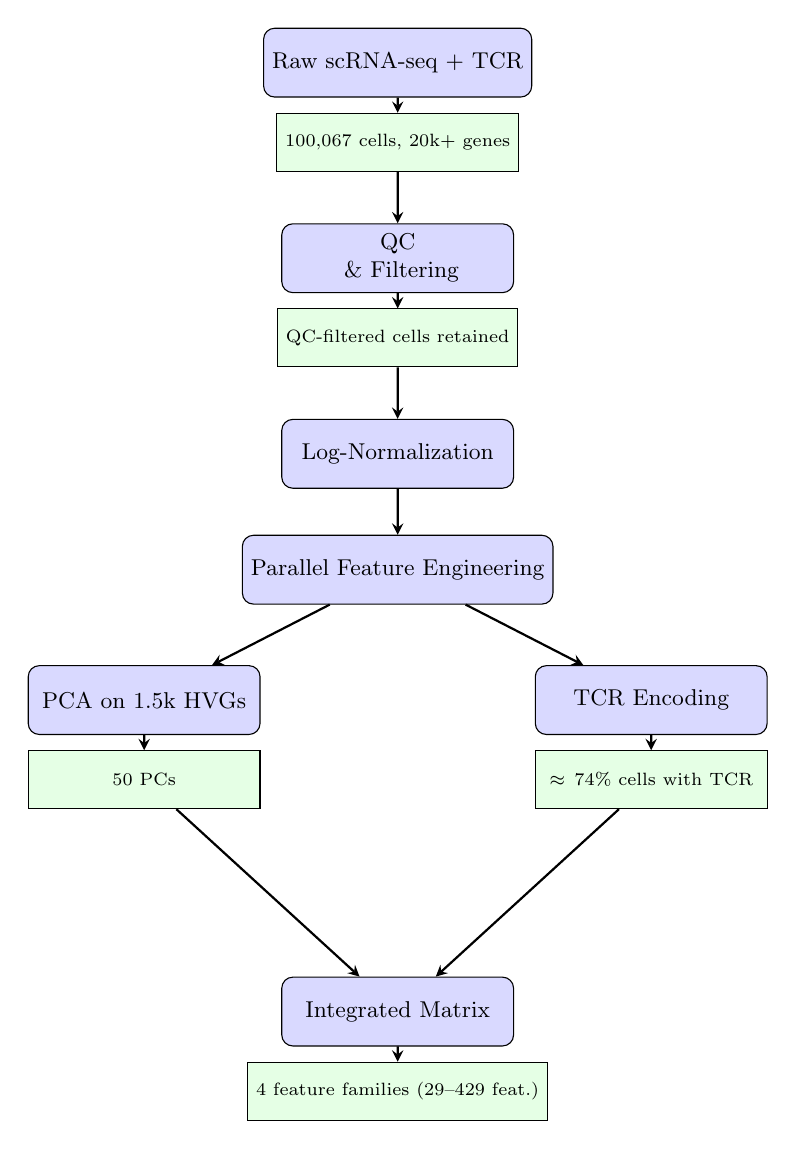
\begin{tikzpicture}[node distance=1.3cm, transform shape, scale=0.92]
    \tikzset{
      process/.style = {rectangle, rounded corners, minimum width=3.2cm, minimum height=0.95cm, align=center, draw=black, fill=blue!15, font=\small},
      data/.style = {rectangle, minimum width=3.2cm, minimum height=0.8cm, align=center, draw=black, fill=green!10, font=\scriptsize},
      arrow/.style = {thick,->,>=stealth}
    }
    
    \node (raw) [process] {Raw scRNA-seq + TCR};
    \node (raw_data) [data, below of=raw, yshift=0.2cm] {100,067 cells, 20k+ genes};
    \node (qc) [process, below of=raw_data, yshift=-0.3cm] {QC \\\ \& Filtering};
    \node (qc_data) [data, below of=qc, yshift=0.2cm] {QC-filtered cells retained};
    \node (norm) [process, below of=qc_data, yshift=-0.3cm] {Log-Normalization};
    \node (split) [process, below of=norm, yshift=-0.3cm] {Parallel Feature Engineering};
    
    \node (pca) [process, below of=split, xshift=-3.5cm, yshift=-0.5cm] {PCA on 1.5k HVGs};
    \node (pca_data) [data, below of=pca, yshift=0.2cm] {50 PCs};
    
    \node (tcr) [process, below of=split, xshift=3.5cm, yshift=-0.5cm] {TCR Encoding};
    \node (tcr_data) [data, below of=tcr, yshift=0.2cm] {$\approx\,74\%$ cells with TCR};
    
    \node (final) [process, below of=split, yshift=-4.8cm] {Integrated Matrix};
    \node (final_data) [data, below of=final, yshift=0.2cm] {4 feature families (29--429 feat.)};
    
    \draw [arrow] (raw) -- (raw_data);
    \draw [arrow] (raw_data) -- (qc);
    \draw [arrow] (qc) -- (qc_data);
    \draw [arrow] (qc_data) -- (norm);
    \draw [arrow] (norm) -- (split);
    \draw [arrow] (split) -- (pca);
    \draw [arrow] (split) -- (tcr);
    \draw [arrow] (pca) -- (pca_data);
    \draw [arrow] (tcr) -- (tcr_data);
    \draw [arrow] (pca_data) -- (final);
    \draw [arrow] (tcr_data) -- (final);
    \draw [arrow] (final) -- (final_data);
\end{tikzpicture}


\end{center}
\vspace{8pt}
\captionof{figure}{Enhanced Data Processing Pipeline with quantitative details at each stage, showing cell counts, feature dimensions, and variance explained.}
\end{minipage}

\end{document}
